\section{Executable authority-revocation contract}

The long-form theory distinguishes two objects that are easy to conflate in an implementation: an append-only history of authority certificates and challenges, and the non-monotone view of certificates that are currently valid. The reference implementation includes a small executable authority-ledger contract that makes this distinction explicit.

An \texttt{AuthorityProposal} carries a claim, one authority axis, a scope and evidence identities but has no active authority. A verifier outcome may mint a scoped \texttt{AuthorityCertificate} only for \texttt{SUPPORTED} or explicitly partial outcomes. Refuted or uncheckable proposals do not change the active authority view. A later \texttt{revoke} operation removes a certificate from the active set while retaining both the certificate and its issue/revocation events in the historical ledger. \texttt{supersede} similarly deactivates an older certificate and activates a replacement without deleting the old record. Figure~\ref{fig:lifecycle} shows the resulting lifecycle.

\begin{figure}[t]
\centering
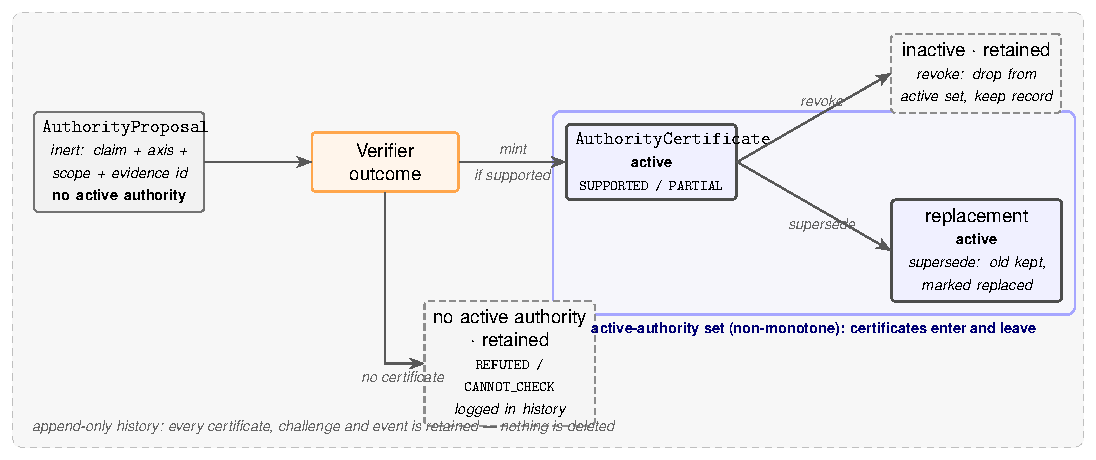
\includegraphics[width=\textwidth]{figures/claim_lifecycle.pdf}
\caption{Lifecycle of a claim through the authority ledger. A proposal is inert until a verifier outcome mints an active certificate for a supported or partial result; refuted and uncheckable proposals acquire no active authority but are retained. Revocation and supersession remove a certificate from the active set without deleting it. The historical ledger is append-only, while the active-authority set is non-monotone: certificates may both enter and leave it. This is exactly the distinction---historical monotonicity without active-authority monotonicity---that the formalism requires.}
\label{fig:lifecycle}
\end{figure}

The implementation is intentionally coordinate-local. Issuing a representation certificate does not create a mechanism certificate, and there is no generic cross-axis coercion function. Any future operation that raises a different authority coordinate must therefore be a separately registered inference rule with its own evidence obligations. The corresponding tests cover proposal non-sovereignty, axis non-escalation, refutation-driven authority decrease, supersession traceability and fail-closed evidence identity.

This module is a reference conformance object, not a claim that Orion invented transactional belief commit. Contemporary agent-memory systems already provide substantially richer transaction, provenance and authorization mechanisms \cite{memtx2026,ppmf2026,tmanm2026,committime2026}. Its role in this paper is narrower: it demonstrates that the scientific distinction used by the authority formalism---historical monotonicity without active-authority monotonicity---has an executable state-transition realization.
